%<*named>
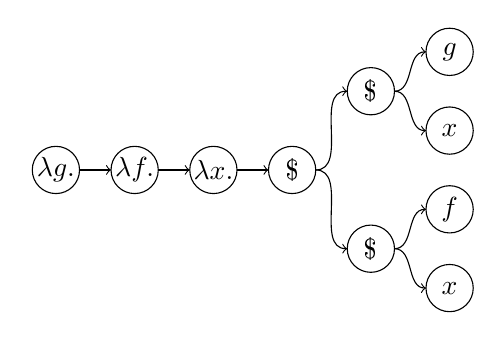
\begin{tikzpicture}
\draw (0,0)    circle (.3cm) node[align=center] {$\lambda{}g.$};
\draw (1,0)    circle (.3cm) node[align=center] {$\lambda{}f.$};
\draw (2,0)    circle (.3cm) node[align=center] {$\lambda{}x.$};
\draw (3,0)    circle (.3cm) node[align=center] {\$};

\draw (4,-1)   circle (.3cm) node[align=center] {\$};
\draw (5,-.5)  circle (.3cm) node[align=center] {$f$};
\draw (5,-1.5) circle (.3cm) node[align=center] {$x$};

\draw (4,1)    circle (.3cm) node[align=center] {\$};
\draw (5,1.5)  circle (.3cm) node[align=center] {$g$};
\draw (5,.5)   circle (.3cm) node[align=center] {$x$};

\draw [->] (0.3,0)   to [out=0,in=180] (0.7,0);
\draw [->] (1.3,0)   to [out=0,in=180] (1.7,0);
\draw [->] (2.3,0)   to [out=0,in=180] (2.7,0);
\draw [->] (3.3,0)   to [out=0,in=180] (3.7,-1);
\draw [->] (3.3,0)   to [out=0,in=180] (3.7,1);
\draw [->] (4.3,1)   to [out=0,in=180] (4.7,1.5);
\draw [->] (4.3,1)   to [out=0,in=180] (4.7,.5);
\draw [->] (4.3,-1)  to [out=0,in=180] (4.7,-1.5);
\draw [->] (4.3,-1)  to [out=0,in=180] (4.7,-.5);
\end{tikzpicture}
%</named>

%<*debruijn>
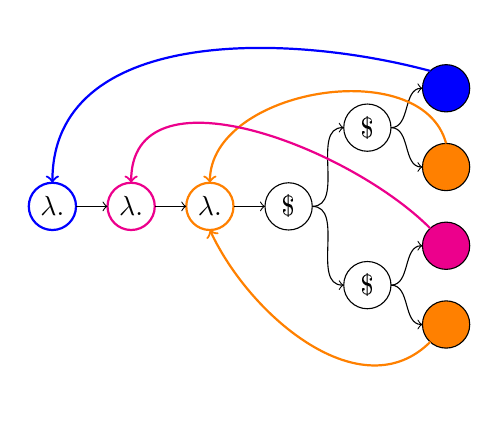
\begin{tikzpicture}
\draw[draw=blue   ,thick] (0,0)    circle (.3cm) node[align=center] {$\lambda{}.$};
\draw[draw=magenta,thick] (1,0)    circle (.3cm) node[align=center] {$\lambda{}.$};
\draw[draw=orange ,thick] (2,0)    circle (.3cm) node[align=center] {$\lambda{}.$};
\draw (3,0)    circle (.3cm) node[align=center] {\$};

\draw               (4,-1)   circle (.3cm) node[align=center] {\$};
\draw[fill=magenta] (5,-.5)  circle (.3cm) node[align=center] {};
\draw[fill=orange]  (5,-1.5) circle (.3cm) node[align=center] {};

\draw              (4,1)    circle (.3cm) node[align=center] {\$};
\draw[fill=blue]   (5,1.5)  circle (.3cm) node[align=center] {};
\draw[fill=orange] (5,.5)   circle (.3cm) node[align=center] {};

\draw [->] (0.3,0)   to [out=0,in=180] (0.7,0);
\draw [->] (1.3,0)   to [out=0,in=180] (1.7,0);
\draw [->] (2.3,0)   to [out=0,in=180] (2.7,0);
\draw [->] (3.3,0)   to [out=0,in=180] (3.7,-1);
\draw [->] (3.3,0)   to [out=0,in=180] (3.7,1);

\draw [->] (4.3,1)   to [out=0,in=180] (4.7,1.5);
\draw[blue, thick] [->] (4.8,1.72)   to [out=165,in=90] (0,.3);

\draw [->] (4.3,1)   to [out=0,in=180] (4.7,.5);
\draw[orange, thick] [->] (5,.8)   to [out=105,in=90] (2,.3);

\draw [->] (4.3,-1)  to [out=0,in=180] (4.7,-.5);
\draw[magenta, thick] [->] (4.8,-.28)   to [out=135,in=90] (1,.3);

\draw [->] (4.3,-1)  to [out=0,in=180] (4.7,-1.5);
\draw[orange, thick] [->] (4.8,-1.72) to [out=225,in=295] (2,-.3);

\end{tikzpicture}
%</debruijn>

%<*codebruijn>
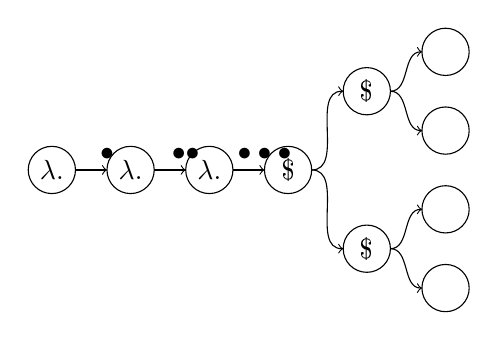
\begin{tikzpicture}
\draw (0,0)    circle (.3cm) node[align=center] {$\lambda{}.$};
\draw (1,0)    circle (.3cm) node[align=center] {$\lambda{}.$};
\draw (2,0)    circle (.3cm) node[align=center] {$\lambda{}.$};
\draw (3,0)    circle (.3cm) node[align=center] {\$};

\draw (4,-1)   circle (.3cm) node[align=center] {\$};
\draw (5,-.5)  circle (.3cm) node[align=center] {};
\draw (5,-1.5) circle (.3cm) node[align=center] {};

\draw (4,1)    circle (.3cm) node[align=center] {\$};
\draw (5,1.5)  circle (.3cm) node[align=center] {};
\draw (5,.5)   circle (.3cm) node[align=center] {};

\draw [->] (0.3,0)   to [out=0,in=180] (0.7,0)  node[above]{$\bullet$};
\draw [->] (1.3,0)   to [out=0,in=180] (1.7,0)  node[above]{$\bullet\bullet$};
\draw [->] (2.3,0)   to [out=0,in=180] (2.7,0)  node[above]{$\bullet\bullet\bullet$};
\draw [->] (3.3,0)   to [out=0,in=180] (3.7,-1);
\draw [->] (3.3,0)   to [out=0,in=180] (3.7,1);
\draw [->] (4.3,1)   to [out=0,in=180] (4.7,1.5);
\draw [->] (4.3,1)   to [out=0,in=180] (4.7,.5);
\draw [->] (4.3,-1)  to [out=0,in=180] (4.7,-1.5);
\draw [->] (4.3,-1)  to [out=0,in=180] (4.7,-.5);
\end{tikzpicture}
%</codebruijn>
